\documentclass[conference]{IEEEtran}
\usepackage{soulutf8}
\usepackage{cite}
\usepackage{amsmath,amssymb,amsfonts}
\usepackage{algorithmic}
\usepackage{graphicx}
\usepackage{textcomp}
\usepackage{xcolor}
\def\BibTeX{{\rm B\kern-.05em{\sc i\kern-.025em b}\kern-.08em
    T\kern-.1667em\lower.7ex\hbox{E}\kern-.125emX}}
\begin{document}

\title{Progetto B1: Multicast totalmente e causalmente ordinato in Go}

\author{\IEEEauthorblockN{Simone Tiberi}
\IEEEauthorblockA{\textit{Corso di "Sistemi Distribuiti e Cloud Computing"} \\
\textit{Università degli Studi di Roma Tor Vergata, facoltà di Ingegneria Informatica}\\
Roma, Italia \\
simone.tiberi.98@gmail.com}
}


\maketitle

\begin{abstract}
L'obiettivo di questo documento è quello di analizzare e descrivere la metodologia adottata nelle varie fasi dello sviluppo del progetto, ponendo particolare enfasi sull'architettura adottata e le scelte implementativi effettuate. 
\end{abstract}

\section{Introduzione}
\textbf{comuniGO} è un'applicazione distribuita sviluppata principalmente in GO che permette ad un insieme di peer connessi ad un gruppo di multicast di comunicare utilizzando diversi algoritmi.

\begin{figure}[htbp]
\centerline{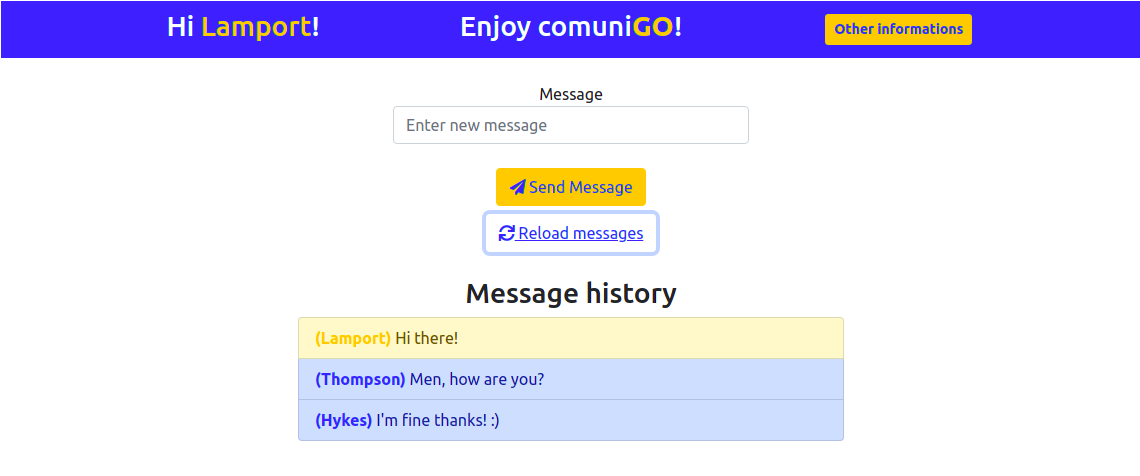
\includegraphics[width=0.4\textwidth]{figs/home.png}}
\caption{Home page di comuniGO}
\label{fig:home}
\end{figure}

L'applicazione soddisfa i requisiti richiesti dalla traccia, ovvero:
\begin{itemize}
\item prevede un servizio di registrazione per i peer che vogliono partecipare al gruppo di multicast, assumendo che la membership sia statica durante l'esecuzione;

\item prevede il supporto dei seguenti algoritmi di multicast:
\begin{enumerate}
\item \ul{multicast totalmente ordinato} implementato in modo centralizzato tramite un \ul{sequencer};

\item \ul{multicast totalmente ordinato} implementato in modo decentralizzato tramite l'uso di \ul{clock logici
scalari};

\item \ul{multicast causalmente ordinato} implementato in modo decentralizzato tramite l'uso di \ul{clock
logici vettoriali}.
\end{enumerate}
\end{itemize}

Inoltre, come richiesto dalla specifica, è stato testato il funzionamento degli algoritmi implementati nel caso in cui:
\begin{itemize}
\item vi sia un solo processo che invia il messaggio di multicast
\item molteplici processi contemporaneamente inviino un
messaggio di multicast;
\end{itemize}
e per simulare condizioni di maggiore stress nel testing è stato incluso, come cconsigliato, un parametro \texttt{delay} configurabile che permette di specificare un ritardo nell'invio generato in modo random in un intervallo predefinito.

Per facilitare il debugging dell'applicazione, come suggerito dalla traccia,  stato implementato un flag di tipo \textit{verbose}, che se attivo stampa informazioni di logging con i dettagli dei messaggi inviati e ricevuti.

\section{Tecnologie adottate}
Per lo sviluppo del progetto si è fatto uso delle seguenti tecnologie:
\begin{itemize}
\item \textbf{Docker} per il supporto alla virtualizzazione;
\item \textbf{Docker compose} per coordinare l'esecuzione dei container sul singolo nodo (e.g. startup, shutdown, interconnessione degli elementi);
\item \textbf{Go} come unico linguaggio per lo sviluppo della logica applicativa;
\item \textbf{gRPC} come framework RPC per lo scambio dei messaggi fra i componenti dell'applicazione;
\item \textbf{Redis} come datastore in memory per la memorizzazione dei messaggi \textit{consegnati a livello applicativo} dai vari algoritmi;
\item \textbf{HTML}, \textbf{Javascript} (\textbf{jQuery}) e \textbf{CSS} per la realizzazione del frontend Web con cui interagire con l'applicazione.
\end{itemize}

\section{Architettura}
\begin{figure}[htbp]
\centerline{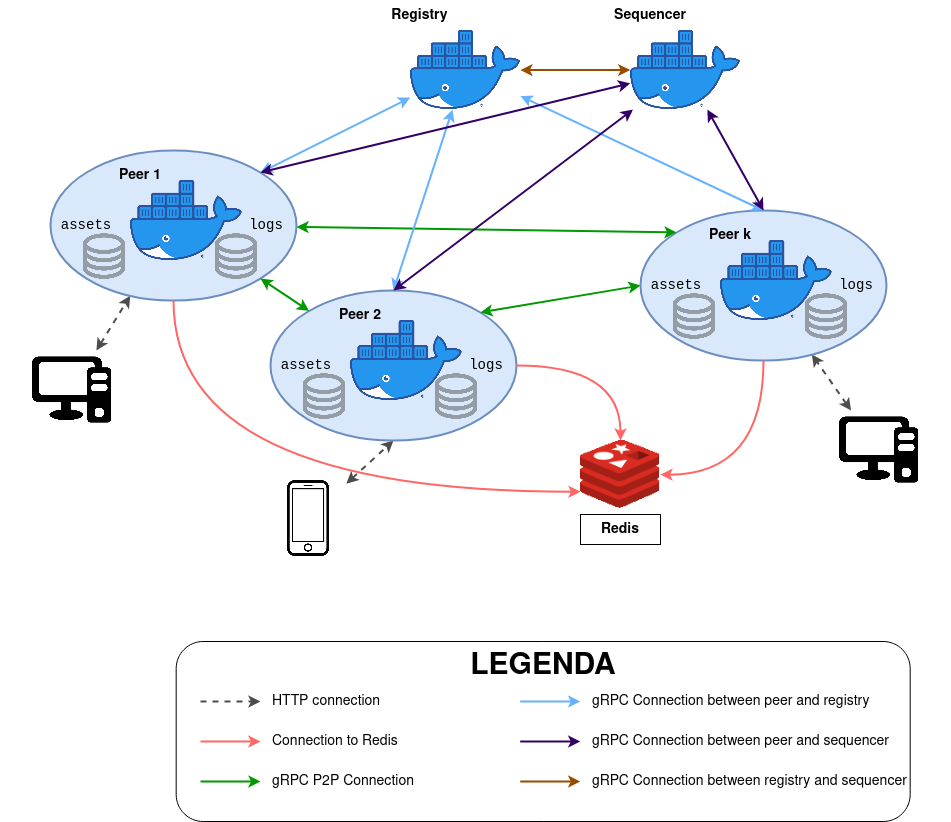
\includegraphics[width=0.4\textwidth]{figs/architecture.png}}
\caption{Architettura realizzata.}
\label{fig:architecture}
\end{figure}

In figura \ref{fig:architecture} è riportata una schematizzazione dell'architettura adottata per lo sviluppo dell'applicazione, in cui è possibile notare come:
\begin{itemize}
\item ciascun \textbf{peer} sia associato ad un volume docker etichettato come \texttt{logs} di tipo \textit{bind} ove avviene la scrittura su file separati sia del log della logica applicativa che delle richieste ricevute dal webserver;

\item ogni peer è interconnesso con un'istanza unica di Redis, un datastore in memory di tipo chiave-valore, per la memorizzazione dei messaggi \textit{consegnabili all'utente};

\item la logica applicativa è interamente realizzata sfruttando il meccanismo RPC per qualunque coppia di endpoint;

\item l'utente finale può scambiare i propri messaggi con gli altri connessi al gruppo di multicast semplicemente utilizzando il proprio browser (o in alternativa sfruttando programmi come \texttt{curl}). 
\end{itemize}
\newpage
\section{Logica applicativa}
\subsection{Registrazione}
\begin{figure}[htbp]
\centerline{
\includegraphics[width=0.4\textwidth]{figs/login.png}}
\caption{Login di comuniGO}
\label{fig:login}
\end{figure}
Lato frontend, la registrazione prevede che:
\begin{enumerate}
\item l'utente si colleghi ad uno dei peer del gruppo, i quali possono essere individuati tramite lo script di discovery o il programma GO apposito, descritti all'interno del README file;
\item inserisca un nome utente unico all'interno del gruppo;
\item attenda che tutti quanti i membri siano realmente connessi prima di entrare effettivamente nel portale di comunicazione.
\end{enumerate}

Lato backend invece:
\begin{enumerate}
\item il peer inoltra al servizio di registrazione l'username ricevuto dal frontend;
\item le procedure remote server-side inviano quanto ricevuto dai peer ad un'apposita go routine che mantiene la lista non ancora completa degli utenti connessi;
\item nel momento in cui si raggiunge la taglia del gruppo prevista, la routine in questione sblocca le procedure in attesa di poter inviare la composizione del gruppo al peer richiedente
\item una volta ricevuta la composizione, il peer la inoltra via HTTP al client web affichè:
\begin{itemize}
\item Si effettui il redirect verso il reale portale per la comunicazione
\item Si mostri un messaggio d'errore ove necessario
\end{itemize}
\end{enumerate}
\subsection{Comunicazione tramite sequencer}
Nel caso in cui la modalità di comunicazione selezionata è quella basata sull'utilizzo di un sequencer, il nodo di registrazione comunica la composizione del gruppo di multicast anche a quest'ultimo prima di terminare la sua esecuzione.

Una volta raggiunto lo \textit{steady state}, ovvero dopo che tutti i peer si sono correttamente registrati e il sequencer abbia ricevuto la lista di peer connessi, la comunicazione tramite il nodo centrale si basa sull'iter di seguito riportato:

\begin{itemize}
\item Nella comunicazione \ul{dal peer al sequencer}
\begin{enumerate}
\item il peer inoltra al seequencer il messaggio ricevuto dal frontend; 
\item le procedure remote server-side inviano quanto ricevuto dai peer ad un'apposita go routine responsabile di Ordinare in modo univoco i messaggi ricevuti e marcarli con un apposito timestamp (\textit{sequence number})
\end{enumerate}

\item Nella comunicazione \ul{dal sequencer al peer} ogni qual volta la go routine dedicata all'ordinamento marca un nuovo messaggio con un determinato timestamp, questo viene inoltrato sulle varie connessioni aperte in precedenza verso tutti i peer
\end{itemize}

\subsection{Comunicazione basata su clock logici scalari}
\subsection{Comunicazione basata su clock logici vettoriali}

\section{Testing}
\section{Deployment su cluster reali}

\end{document}
